\documentclass[../main.tex]{subfiles}
\graphicspath{{\subfix{../images/}}}

\begin{document}
As it turns out, there's more to algebra than pure uninspiring symbol pushing. In this chapter we look at some structures and concepts in elementary algebra.

\begin{figure}[H]
    \centering
    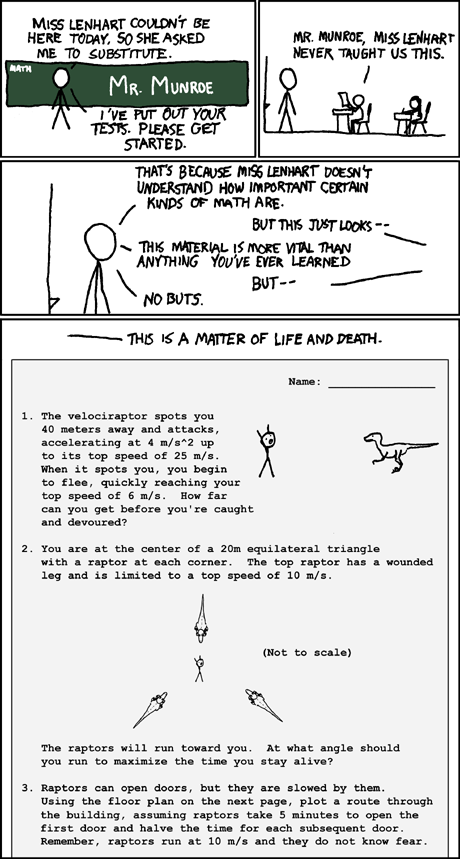
\includegraphics[scale=0.5]{xkcd_substitute.png}
    \caption{Comic from https://xkcd.wtf/135/}
\end{figure}

\subsection{Many Manipulations}
\subsubsection{Factorising and Re-expressing}
Starting off easy, we will explore some funny-looking problems that solve themselves after some smart rearranging and rewriting.

\begin{example}[2013 SMO(J) P15]
    If $a=1.69$, $b=1.73$ and $c=0.48$, find the value of
    $$\frac{1}{a^2-ac-ab+bc}+\frac{2}{b^2-ab-bc+ac}+\frac{1}{c^2-ac-bc+ab}.$$
\end{example}
Of course, a good calculator can do this in seconds (although typing it in may take longer...), but what if you had to do this by hand? Substituting may not be smart...

However, we note that each of the denominators are suspiciously factorisable. For example,
$$a^2-ac-ab+bc=a(a-c)-b(a-c)=(a-b)(a-c).$$

\begin{proof}
    Hence,
\begin{align*}
    & \frac{1}{a^2-ac-ab+bc}+\frac{1}{b^2-ab-bc+ac}+\frac{1}{c^2-ac-bc+ab}\\
    &=\frac{1}{(a-b)(a-c)}+\frac{2}{(b-c)(b-a)}+\frac{1}{(c-b)(c-a)} \\
    &=\frac{(b-c)-2(a-c)+(a-b)}{(a-b)(a-c)(b-c)} \\
    &=-\frac{1}{(a-b)(b-c)} = -\frac{1}{(-0.04)(1.25)} = \boxed{20}
\end{align*}
\end{proof}


\begin{example}[2013 SMO(J) P32]
    If $a$ and $b$ are positive integers such that $a^2+2ab-3b^2-41=0$, find $a^2+b^2$.
\end{example}
The constant "$41$" seems irrelevant to the equation at this point, except that it's a prime number (this may be important!). For now, let us write the equation as $a^2+2ab-3b^2=41$.

\begin{proof}
    Notice that the coefficients of the LHS sum to $(1+2-3=)0$(!), so this tells us that we should factorise:
$$a^2+2ab-3b^2=a^2-ab+3ab-3b^2=a(a-b)+3b(a-b)=(a+3b)(a-b)=41.$$

Now, it becomes apparent why $41$ was chosen: because it is a prime number, and $a,b$ are integers, $a+3b$ and $a-b$ are each either $1$ or $41$. Moreover, $a+3b \geq a-b$ so we have
$$
\begin{cases}
    a+3b&=41 \\
    a-b&=1
\end{cases} \implies a=11, b=10.
$$
Thus, $a^2+b^2=11^2+10^2=\boxed{221}$.
\end{proof}


\begin{example}[2017 SMO(J) P20]
    Let $a$, $b$ and $c$ be positive integers such that
    $$a^2+bc=257\quad\text{and}\quad ab+bc=101.$$

    Find the value of $a$, $b$ and $c$.
\end{example}
\begin{proof}
    Armed with the idea from the previous problem, we see again that $101$ is a prime number, so $b(a+c)=101$. Moreover, $b+c\geq a$ so that $b=1$ and $a+c=101$. Thus, $$a^2+bc=a^2+c=a^2+(101-a)=257 \implies a(a-1)=156.$$

    With some guess and check (since $a$ is a positive integer), $a=13$, $b=1$ and $c=88$.
\end{proof}


\begin{example}[2016 SMO(J) P24]
    If $\frac{a}{2b}=\frac{2b}{3c}=\frac{3c}{8a}$, find the value of $\frac{ac+cb}{cb-ba}.$
\end{example}
The given condition tells us that $a$, $b$ and $c$ are all connected, so we should express $a$ and $b$ in terms of $c$.

\begin{proof}
    Let $\frac{a}{2b}=\frac{2b}{3c}=\frac{3c}{8a}=k$ for some real $k$. We have
$$ 
\begin{cases}
    a=2kb \\
    2b=3kc \\
    3c=8ka
\end{cases}
\implies
\begin{cases}
    a=3k^2c \\
    2b=8k^2a \\
\end{cases}
\implies
\begin{cases}
    a=24k^5c \\
    b=12k^4c    
\end{cases} 
.$$
By the given condition, we have $\frac{2b}{3c}=\frac{24k^4c}{3c}=8k^4=k \implies 8k^3=1 \implies k=\frac{1}{2}$, $k^5=\frac{1}{32}$

Hence,
\begin{align*}
    \frac{ac+cb}{cb-ba}
    &= \frac{24k^5c^2+12k^4c^2}{12k^4c^2-288k^9c^2} \\
    &= \frac{2k+1}{1-24k^5} \\
    &= \frac{2\cdot\frac{1}{2}+1}{1-24\cdot\frac{1}{32}} = \boxed{8}
\end{align*}
\end{proof}

For the first substantial technique of this section, we introduce the trick of \textit{counting degrees}.

\begin{proposition}[Counting degrees]
    We say that an expression or equation is \textit{homogenous} (or homogenised) if there is no loose constant terms remaining. For example, $x^3+2022x^2y+2021$ is non-homogenous because of the constant $2021$, while $x^3+2022xy^3+xy$ is homogenous because there is no loose constant. 

    We \textit{want} to work with homogenous expressions because degrees cancel nicely, and expressions are usually neat. 
\end{proposition}
\begin{example}
    If $x$ and $y$ are real numbers such that $x+y=2$ and that
    $$\frac{(1-x)^2}{x}+\frac{(1-y)^2}{y}=-4,$$
    find the value of $xy$.
\end{example}

Consider the term $\frac{(1-x)^2}{x}$. The numerator is a quadratic (degree $2$) while the denominator is linear (degree $1$), so we say that this term is of degree $1$. The term $\frac{(1-y)^2}{y}$ is also similarly of degree $1$, and so the LHS is of degree $1$. 

On the other hand, the RHS is a constant (degree $0$), which makes the equation \textit{non-homogenous}. Fortunately, we are given that $x+y=2$. 

\begin{proof}
    We begin by writing
$$\frac{(1-x)^2}{x}+\frac{(1-y)^2}{y}=-2(x+y).$$ Now, our equation is homogenous, and as we shall see, this equation now resolves itself very cleanly. Clearing denominators (since $x,y \neq 0$), we have
\begin{align*}
    \frac{(1-x)^2}{x}+\frac{(1-y)^2}{y}=-2(x+y) &\implies x(1-y)^2+y(1-x)^2=-2xy(x+y) \\
    &\implies (xy^2-2xy+x)+(x^2y-2xy+y)=-2x^2y-2xy^2 \\
    &\implies 3x^2y+3xy^2-4xy+(x+y)=0 \\
    &\implies 3xy(x+y)-4xy+(x+y)=0 \\
    &\implies 2xy+2=0 \implies xy=\boxed{-1}
\end{align*}
\end{proof}

\subsubsection{Substitutions}
Sometimes scary expressions are just expanded versions of simpler expressions! A smart substitution reduces a large amount of gruntwork, and simplifies things nicely.

To start off, we showcase an application of a nifty substitution, without which, the problem may be untractable to the unsuspecting student.
\begin{example}[2013 SMO(J) P11]
    Find the value of $\sqrt{9999^2+19999}.$
\end{example}
Certainly, we are not expected to multiply out and then take the square root of this monstrous expression! However, we do note that the choice of $9999$ is completely arbitrary, so it may be wise to make a substitution for $9999$ and express $19999$ in terms of $a$.

\begin{proof}
    Let $a=9999$, then $19999=2\cdot 9999+1=2a+1$. Aha! We now know
\begin{align*}
    \sqrt{9999^2+19999}&=\sqrt{a^2+(2a+1)} \\
    &=\sqrt{(a+1)^2}=a+1 \\
    &=\boxed{10000}.
\end{align*}
How nice!
\end{proof}

\begin{example}[2014 SMO(J) P16]
    Let $m$ and $n$ be positive real numbers satisfying the equation
    $$m+4\sqrt{mn}-2\sqrt{m}-4\sqrt{n}+4n=3.$$
    Find the value of $$\frac{\sqrt{m}+2\sqrt{n}+2014}{4-\sqrt{m}-2\sqrt{n}}.$$
\end{example}
The required value is just as grizzly as the given equation. To start, we should be somewhat suspicious of the term $4\sqrt{mn}$: this is a term of degree $1$, since $\sqrt{m}$ and $\sqrt{n}$ both have degree $\frac{1}{2}$. Yet, it's mixed in an expression containing terms of degree $\frac{1}{2}$ like $2\sqrt{m}$ and $4\sqrt{n}$, as well as degree $1$ terms like $m$ and $4n$.

This strongly suggests the substitutions $x=\sqrt{m}, y=\sqrt{n}$, so we want the value of 
$$\frac{\sqrt{m}+2\sqrt{n}+2014}{4-\sqrt{m}-2\sqrt{n}}=\frac{x+2y+2014}{4-(x+2y)}.$$

The given equation gives $$x^2+4xy-2x-4y+4y^2=3. \implies (x+2y)^2-2(x+2y)=3 \implies (x+2y)(x+2y-2)=3.$$ Setting $z=x+2y$, $z(z-2)=3 \implies z^2-2z-3=0 \implies z=3$ only since $z=x+2y>0$. 

Hence, the required value is \boxed{4}.

\begin{example}[2015 SMO(J) P21]
    Find the value of $$\sqrt{(98\cdot 100+2)(100\cdot 102+2)+(100\cdot 2)^2}.$$
\end{example}
Once again, this is a monstrous expression, but fortunately the individual parts in the expression are broken down slightly for us. For now, let us focus on the term $98\cdot 100+2$. 

It may be tempting to simply substitute $a=98$ (or $a=100$), but the expression $a(a+2)+2=a^2+2a+2$ is cumbersome to work with. Perhaps we should compromise and let $a=99$ instead!

Then, $98\cdot 100+2= (a-1)(a+1)+2=a^2+1=99^2+1$, and similarly, $100\cdot 102+2 = 101^2+1$. The desired expression is now
$\sqrt{(99^2+1)(101^2+1)+(100\cdot 2)^2}$, and it is apparent why $100\cdot 2$ was written instead of $200$. Letting $b=100$, we have
\begin{align*}
    \sqrt{(99^2+1)(101^2+1)+(100\cdot 2)^2}&=\sqrt{((b-1)^2+1)((b+1)^2+1)+4b^2}\\
    &=\sqrt{(b^2-2b+2)(b^2+2b+2)+4b^2}=\sqrt{((b^2+2)-2b)((b^2+2)+2b)+4b^2} \\
    &=\sqrt{(b^2+2)^2-(2b)^2+4b^2} \\
    &= b^2+2=\boxed{10002}
\end{align*}

\subsection{Polynomials}
Outside of quadratic polynomials, there are also cubics, quartics, quintics, sextics..., that most students assume are extinct. However, they can be found in a select number of natural hideouts!

\subsubsection{Quadratics}
In this section, we will revisit the common quadratic polynomials.
The techniques for quadratics aren't many. The usual few are the discriminant and completing the square, none of which are totally unexpected or inspiring. However, they are still useful-ish in extracting information from a given problem. We hope it suffices!
\begin{example}[2010-2011 Mandelbrot]
    Let $P(x)=x^3+ax^2+bx+c$ be a polynomial with three distinct roots. The polynomial P(Q(x)), where $Q(x)=x^2+x+2001$, has no real roots. Prove that $P(2001)>\frac{1}{64}$.
\end{example}
This is a strange idea: given the number of roots of a polynomial, what can we deduce about it's value?

\begin{proof}
    For starters, let $p,q,r$ be the three distinct roots of $P$, then $P(x)=(x-p)(x-q)(x-r)$ and let $z$ be a complex root of $P(Q(x))$ so that $P(Q(z))=0$. 

Hence, $Q(z)=\text{$p$ or $q$ or $r$}$. Without loss of generality, $$Q(z)=p \implies z^2+z+(2001-p)=0.$$

However, there are no real values of $z$ that satisfy this condition! This next step would be glaring: by considering the discriminant,
$$\Delta=1-4(2001-p) < 0 \implies p < \frac{8003}{4}.$$

Since we initially assumed without loss of generality that $Q(z)=p$, this conclusion should also hold for $q, r$, that is $p,q,r < \frac{8003}{4}$.

Finally, \begin{align*}
    P(2001)=(2001-p)(2001-q)(2001-r) &> \frac{1}{4}\cdot\frac{1}{4}\cdot\frac{1}{4} \\
    &=\frac{1}{64}
\end{align*}
\end{proof}
Next, we consider a quadratic with coefficients that form an arithmetic progression. As it turns out, if the quadratic has a unique root, then we can uniquely determine this root!
\begin{example}[2013 AMC 10B P19]
    Let $c,b,a$ be real numbers form an arithmetic progression with $a\geq b\geq c\geq 0$. The quadratic $ax^2+bx+c=0$ has exactly one root. Find this root.
\end{example}
First step! The discriminant: $\Delta=b^2-4ac=0$, implying that the only root is $x=\frac{-b}{2a}$ by considering the quadratic formula.

\begin{proof}
    Since $c,b,a$ have common differences with $b$ being the median element, we may write $c=b+(b-a)=2b-a$ so that 
$$b^2-4ac=b^2-4a(2b-a)=b^2-8ab+4a^2=0 \implies b=4a\pm2a\sqrt{3}.$$
Yet, we are given that $a\geq b$, so surely $b=4a-2a\sqrt{3}$, giving $x=-\frac{b}{2a}=\boxed{-2+\sqrt{3}}.$
\end{proof}

\subsubsection{The Rare Types}
Contrary to popular belief, there are higher degree polynomials in the wild. We first consider some identities associated with the coefficients of a general polynomial.

Consider a general polynomial $$P(x)=a_nx^n+a_{n-1}x^{n-1}+\cdots+a_1x+a_0$$ with real coefficients $\{a_n\}$. Then, the
\begin{enumerate}
    \item constant term is $P(0)$,
    \item sum of coefficients is $P(1)$,
    \item sum of \textit{odd-power} coefficients is $\frac{P(1)-P(-1)}{2}$,
    \item sum of \textit{even-power} coefficients is $\frac{P(1)+P(-1)}{2}$.
\end{enumerate}

The reader is strongly encouraged to derive the four properties above!

For the other coefficients, there are other higher-powered techniques (pun fully intended) to deal with them, but we will not introduce them here (for the interested, see the roots of unity filter).

We are guessing the student is familiar with the so-called "sum and product of roots" for a quadratic, and here, we introduce a generalisation - we have similar relations for higher-degree polynomials! This is given by Vieta's Theorem.

\begin{proposition}[Vieta's Theorem]
    A general polynomial $P(x)=a_nx^n+a_{n-1}x^{n-1}+\cdots+a_1x+a_0$ with real coefficients $\{a_n\}$ and real and complex roots $r_1, r_2, \cdots r_n$ has the following relations:
    \begin{align*}
        r_1+r_2+\cdots+r_n&=-\frac{a_{n-1}}{a_n}\\
        (r_1r_2+r_1r_3+\cdots+r_1r_n)+(r_2r_3+r_2r_4+\cdots+r_2r_n)+\cdots+r_{n-1}r_n&=\frac{a_{n-2}}{a_n} \\
        r_1r_2\cdots r_n=(-1)^n\frac{a_0}{a_n}
    \end{align*}
    In general, the \textit{sum of roots taken k at a time} is given by $(-1)^k\frac{a_{n-k}}{a_n}.$ Each of these sums are also known as \textit{elementary symmetric polynomials}.
\end{proposition}

Let us show some examples of Vieta's theorem in action. 
\begin{example}[2001 All-Russian Olympiad]
    The equation $(x-\sqrt[3]{13})(x-\sqrt[3]{53})(x-\sqrt[3]{103})=\frac{1}{3}$ has three distinct roots $r,s,t$. Find the value of $r^3+s^3+t^3$.
\end{example}

First of all... yikes! Cube roots and cubes. However, it seems that the three cube roots look arbitrary: while the answer depends on their values, we can find an expression for $r^3+s^3+t^3$ in terms of these cube roots without caring about their values just yet. 
\begin{proof}
    We make the substitution $a=\sqrt[3]{13}$, $b=\sqrt[3]{53}$, $c=\sqrt[3]{103}$, so that our equation is transformed into $$(x-a)(x-b)(x-c)-\frac{1}{3}=0$$. By Vieta's theorem, 
\begin{align*}
    r+s+t&=a+b+c \\
    rs+st+rt&=ab+bc+ca \\
    rst&=abc-\frac{1}{3}.
\end{align*}
Now, how do we use this to our advantage to find $r^3+s^3+t^3$? For starters, we may expand
$$(r+s+t)^3=r^3+s^3+t^3+3r^2s+3r^2t+3rs^2+3rt^2+3s^2t+3st^2+6rst.$$
We're close to finding something substantial - if we can simplify the sum of the terms in the form $m^2n$. A natural way to do this is to expand
$$(r+s+t)(rs+st+rt)=r^2s+r^2t+rs^2+rt^2+s^2t+st^2+3rst.$$

Aha! Now our expression simplifies nicely:
$$(r+s+t)^3=r^3+s^3+t^3+3(r+s+t)(rs+st+rt)-3rst,$$
whence upon arranging, we have
\begin{align*}
    r^3+s^3+t^3
    &=(\alpha+\beta+\gamma)^3-3(\alpha+\beta+\gamma)(\alpha\beta+\beta\gamma+\gamma\alpha)+3(\alpha+\beta+\gamma+\frac{1}{3})\\
    &=(\alpha+\beta+\gamma)^3-3(\alpha+\beta+\gamma)(\alpha\beta+\beta\gamma+\gamma\alpha)+3(\alpha+\beta+\gamma)+1 \\
    &=\alpha^3+\beta^3+\gamma^3+1 \\
    &=\boxed{170}
\end{align*}
\end{proof}

\begin{example}[2019 AIME I P10]
For complex numbers $z_1, z_2,\cdots z_{673}$, the polynomial
$$(x-z_1)^3(x-z_2)^3\cdots(x-z_673)^3$$
can be expressed as $x^{2019}+20x^{2018}+19x^{2017}+g(x)$ where $g(x)$ is a polynomial with complex polynomials and of degree \textit{at most} $2016$. Find the value of 
$$\sum_{1\leq j\leq k\leq 673}z_jz_k.$$
\end{example}
The sum requested of us is an elementary symmetric polynomial, so we would expect to use Vieta's theorem in some way.

Let $S, P$ denote the sum of roots one and twice at a time respectively and let $Q(x)$ denote the given polynomial. Note that the required sum is $P$. Since it's weird that the given polynomial is cubed throughout, we shall consider
$$p(x)=(x-z_1)(x-z_2)\cdots(x-z_{673})=x^{673}-Sx^{672}+Px^{671}+\cdots$$

Thus, $Q(x)=[p(x)]^3$. To find $S$ and $P$, we shall expand this to find the coefficients of $x^{2018}$ and $x^{2017}$. To do this quickly, we consider how terms in 3 products can be multiplied together to give the relevant terms.

To wit, 
\begin{enumerate}
    \item $x^{2019}$ can only be formed by multiplying all three $x^{673}$, and there is only 1 way to do this.
    \item $x^{2018}$ can be formed by multiplying two $x^{673}$ and one $Sx^{672}$, and there are $\binom{3}{1}=3$ ways to do this.
    \item $x^{2017}$ can be formed by multiplying two $x^{673}$ and one $Px^{671}$, and there are $\binom{3}{1}=3$ ways to do this. It can also be formed by multiplying one $x^{673}$ and two $Sx^{672}$, giving $3$ ways as well.
\end{enumerate}
\begin{proof}
    We now have,
\begin{align*}
    Q(x)=[p(x)]^3&=(x^{673}-Sx^{672}+Px^{671}+\cdots)(x^{673}-Sx^{672}+Px^{671}+\cdots)(x^{673}-Sx^{672}+Px^{671}+\cdots) \\
    &= x^{2019}-3Sx^{2018}+3(P+S^2)x^{2017}+g(x),
\end{align*}
and thus
$$\begin{cases} -3S=20 \\ 3(P+S^2)=19 \end{cases}\Rightarrow \begin{cases} S=-\frac{20}{3} \\ P=-\frac{343}{9}\end{cases}.$$

Hence, $\boxed{P=-\frac{343}{9}}$.
\end{proof}

At this point, it's only complete if we also derive some common algebraic identities and factorisations. 
\begin{proposition}[Classic]
    In what follows, assume the summation run over $x_1,x_2,\cdots,x_n$.
    \begin{enumerate}
        \item For the bivariate $x^2+y^2=(x+y)^2-2xy$, we also have the three-variable relation $$x^2+y^2+z^2=(x+y+z)^2-2(xy+yz+zx).$$
        In general, $$\left(\sum x_i\right)^2=\sum x_i^2-2\left(\sum_{1\leq i\leq q\leq n}x_ix_j\right).$$

        \item $x^3+y^3+z^3-3xyz=\frac{1}{2}(x+y+z)[(x-y)^2+(y-z)^2+(z-x)^2]$.
        This also implies $$x^3+y^3+z^3 \geq 3xyz$$, because
        $(x-y)^2+(y-z)^2+(z-x)^2\geq 0$.
        \item Sophie-Germain Identity: $a^4+4b^4=(a^2+2b^2+2ab)(a^2+2b^2-2ab)$.
        \item Lagrange's Identity: $(a^2+b^2)(c^2+d^2)=(ac-bd)^2+(ad+bc)^2=(ac+bd)^2+(ad-bc)^2$
        \item $(a+b)^3-(a^3+b^3)=3ab(a+b)$.
        \item $(a+b)^5-(a^5+b^5)=5ab(a+b)(a^2+ab+b^2)$.
        \item $(a+b)^7-(a^7+b^7)=7ab(a+b)(a^2+ab+b^2)^2$.
        \item My personal favourite: $\frac{(a^2+bc)(b^2+ac)}{(a+c)(b+c)}+\frac{(a^2+bc)(c^2+ab)}{(a+b)(b+c)}+\frac{(b^2+ac)(c^2+ab)}{(a+b)(a+c)}=a^2+b^2+c^2$
    \end{enumerate}
\end{proposition}
\begin{example}[2016 SMO(O) P15]
    Let $p,q$ be integers such that the roots of the polynomial $f(x)=x^3+px^2+qx-343$ are real. Find the minimum value of $|p^2-2q|$.
\end{example}
This question reeks of Vieta's theorem... With some foresight, we first derive a corollary of the AM-GM inequality for three variables. From identity 2, we know that
    $$x^3+y^3+z^3 \geq 3xyz.$$

    Now take $x=a^{\frac{2}{3}}, y=b^{\frac{2}{3}}, z=c^{\frac{2}{3}}$ so that
    $$a^2+b^2+c^2\geq 3\sqrt[3]{(abc)^2}.$$
    \textit{(whispers) This is a secret tool that will help us later!}
\begin{proof}
    
    Let $a,b,c$ be the real roots of $f$, then by Vieta's theorem, $p=-(a+b+c), q=ab+bc+ca, 343=abc$.
    Thus,
    \begin{align*}
        |p^2-2q|&=|(a+b+c)^2-2(ab+bc+ca)| \\
        &=|a^2+b^2+c^2| \\
        &\geq |3\sqrt[3]{(abc)^2}| = |3\sqrt[3]{343^2}| \\
        &=\boxed{147}
    \end{align*}
\end{proof}

For the final problem of this chapter, we shall prove identity 7.
\begin{example}[Classic]
    Factorise $(a+b)^7-(a^7+b^7)$.
\end{example}
\begin{proof}
    Certainly we need some observations to reduce this problem into a more tractable form. We note that $a=0$ or $b=0$ make the expression vanish, so $ab$ is a factor of the expression. Moreover, since the degrees on $a, b$ are odd, $a=-b$ also causes the expression to vanish. Thus, $a+b$ is also a factor.

    Thus, the expression is a polynomial that readily decomposes into the factor $ab(a+b)$ of degree $3$ and another factor of degree $4$ (or possibly more factors).

    Let $a,b,c$ be roots of the cubic with $c=-(a+b)$ such that
    $$\begin{cases}
        A&=a+b+c=0 \\
        B&=ab+bc+ca=-(a^2+b^2+ab) \\
        C&=abc=-ab(a+b)
    \end{cases},$$
    whence the cubic is $$x^3+Bx-C=(x-a)(x-b)(x-c).$$
    
    This gives $a^2+b^2+c^2=(a+b+c)^2-2(ab+bc+ca)=-2B$. We now "lift" the power up to $x^7$. Suppose $t$ is one of $a,b,c$. Thus, we have
    \begin{align}
        t^7&=t(C-Bt)^2=B^2t^3-2BCt^2+C^2t \\
        &=B^2(C-Bt)-2BCt^2+C^2t \\
        &=-2BCt^2+(C^2-B^3)t+B^2C \label{12-seventh}
    \end{align}
    Summing \eqref{12-seventh} over $t=a,b,c$,
    \begin{align*}
        a^7+b^7-(a+b)^7&=-2BC(-2B)+3B^2C\\
        &=7B^2C=-7ab(a+b)(a^2+ab+b^2)^2
    \end{align*}
    whence $$(a+b)^7-(a^7+b^7)=7ab(a+b)(a^2+ab+b^2)^2.$$
\end{proof}

\subsection{Some Solving}
Many questions will demand you to "find all X satisfying condition Y", the keyword being \textbf{find all}. These problems come in solving equations, functional equations, inequalities, etc. This implies that there are two parts to the problem: 
\begin{enumerate}
    \item Find the solutions and show that no other solutions exist.
    \item Prove that your solutions satisfy the condition (this is part of the problem!).
\end{enumerate}
It will be more instructive for us to work through a problem.

\begin{example}[2021 SMO(O) P10]
Find all real roots to the equation
$$\sqrt[9]{x^7+30x^5}=\sqrt[7]{x^9-30x^5}.$$
\end{example}
As a first scout, we see that $x=0$ is a solution. Moreover, if $x=k$ is a solution, then so is $x=-k$, so we may consider only $x > 0$.
\begin{proof}
Let $a=\sqrt[9]{x^7+30x^5}$, $b=\sqrt[7]{x^9-30x^5}$ so that
$$\begin{cases}
    a-b=0 \\
    a^9+b^7=x^{16}
\end{cases}
\implies
a^{16}=x^{16} \implies a=\pm x.$$

If $a=x$, then $a^9=a^7+30a^5.$ 

Aha! This gives our first solution $a=0$, corresponding to $x=0$. In what follows, we assume $x\neq 0 \implies a\neq 0$.

Thus, $a^4=a^2+30 \implies (a^2-6)(a^2-5)=0 \implies a=\pm \sqrt{5}, a=\pm \sqrt{6}$.

Now, are all of these valid solutions? We should verify so. Suppose $a=x=\sqrt{5}$ (since we have $x>0$), then 
$$a^9=625\sqrt{5}=125\sqrt{5}+750\sqrt{5}=875\sqrt{5},$$ which is a contradiction. Thus $x\neq \sqrt{5}$.
\begin{remark}
Notice the use of proof by contradiction here! We assumed that $x=\sqrt{5}$ is a solution, and then derived the absurd statement that $625\sqrt{5}=875\sqrt{5}$.
\end{remark}
Similarly, suppose $a=x=\sqrt{6}$, then $a^9=1296\sqrt{6}=216\sqrt{6}+1080\sqrt{6}$, which is consistent. Hence, $a=\sqrt{6}$ is the solution we're after. Having exhausted all cases, and verified that our solution was correct, we can now confidently say that the only solutions to the original equation are $$\boxed{\text{$x=0$, $\sqrt{6}$ and $-\sqrt{6}$}}.$$
\end{proof}

Before we go further, we note that sometimes a polynomial is  hard to factorise, especially if it has high degrees or have large coefficients. The Rational Root Theorem is extremely useful to help us discover any potential linear factors and rational roots.
\begin{proposition}[Rational Root Theorem]
For a polynomial $P(x)=a_nx^n+a_{n-1}x^{n-1}+\cdots+a_1x+a_0$ with real coefficients $\{a_n\}=0$, if $P(x)$ \textit{has a rational root} $x=\frac{p}{q}$ where $\gcd(p,q)=1$, then
\begin{itemize}
    \item $p$ is an integer factor of the constant term $a_0$, and
    \item $q$ is an integer factor of the leading coefficient $a_n$.
\end{itemize}
It is important to point out that this \textbf{does not} guarantee that $P(x)$ has a rational root. It merely proposes that there are candidates.
\end{proposition}

Let's see it in action:
\begin{example}[2021 SMO(S) P22]
Find all real solutions $(x,y)$ to the system
\begin{align}
    x^3+y^3+y^2&=0 \label{13-sys-1} \\
    x^2+x^2y+xy^2&=0 \label{13-sys-2}
\end{align}
\end{example}
This is a tough system: both equations are cubic in nature. As an initial scout, it's wise to guess a few solutions: since $x$ is the "lone variable" in equation 2, letting $x=0$ gives $y=0, -1$. We also see that $x=y$ is another solution. In particular, if $x=y$, we have $$2y^3+y^2=0 \implies y=0, -\frac{1}{2}.$$

Thus, we immediately have the solutions $(0,0)$, $(0,-1)$ and $(0, -\frac{1}{2})$, and we know these are (likely) all the solutions because the system has degree 3 (we still need to verify whether there are other nontrivial classes of solution).

\begin{proof}
    To start, we see that \eqref{13-sys-2} is a quadratic in $x$, so $x^2(1+y)+xy^2=0.$ If $x=0$, then we get the three solutions as above. If $y=-1$ in \eqref{13-sys-1}, we have $x=0$, as above. So, suppose $x\neq 0, y\neq -1$, then
$$x(1+y)+y^2=0 \implies x=-\frac{y^2}{1+y}.$$

Putting this into \eqref{13-sys-1}, 
$$-\frac{y^6}{(1+y)^3}+y^2(1+y)=0 \implies \frac{-y^6+y^2(1+y)^3}{(1+y)^4}=0 \implies 4y^3+6y^2+4y+1=0.$$

To factorise this, we use the rational root theorem. The potential roots are thus $y=\pm 1, \pm \frac{1}{2}, \pm\frac{1}{4}$, and from our scouting, we know $y=-\frac{1}{2}$ is a root. Thus,
$$4y^3+6y^2+4y+1=0=(2y+1)(2y^2+2y+1)=0,$$
where the quadratic factor has no real solutions to it. Thus, having exhausted all cases, we have recovered the solutions
$$\boxed{(x,y)=(0,0), (0,-1), (0,-\frac{1}{2})}.$$
\end{proof}

This next problem showcases the mixing of algebra and a string of divisibility arguments. Keep an eye out for these, especially if we are solving over the integers!
\begin{example}[2018 SMO(O) P9]
    Let $p(x)=x^3+ax^2+bx+c$ be a polynomial where $a,b,c$ are distinct non-zero integers. Suppose $p(a)=a^3$ and $p(b)=b^3$. Find $p(13)$.
\end{example}
Hmm, somehow we are apparently able to determine the cubic with only 2 given points. Perhaps the distinct and integer condition will come into play somehow. (For the astute reader, this matches the four degrees of restriction we need to determine a cubic - just as we need four points to determine a cubic as well.)
\begin{proof}
    Given $p(a)=a^3$ and $p(b)=b^3$, we have 
    \begin{align*}
        a^3+ab+c&=0\\
        (a+1)b^2+c&=0
    \end{align*}
    Eliminating $c$,
    we have $(a+1)b^2-ab-a^3=0$, which is a quadratic in $b$.
    
    Using the quadratic formula,
    \begin{align*}
        b&=\frac{a\pm \sqrt{a^2+4a^3(a+1)}}{2(a+1)}\\
        &=\frac{a\pm a\sqrt{4a^2+4a+1}}{2(a+1)}=\frac{a\pm a(2a+1)}{2(a+1)} \\
        &=a \quad \textbf{or} \quad -\frac{a^2}{a+1}
    \end{align*}
    Since $a,b$ are distinct, we must have $b=-\frac{a^2}{a+1}.$
    Moreover, since $b$ is an integer, 
    $$b=-\frac{a^2}{a+1}=-(a-1)-\frac{1}{a+1}$$
    is also an integer. This means $a+1|1 \implies a+1=\pm 1$, giving $a=-2$ only. Thereafter, $b=4$ and $c=16$ follows easily, whence the answer is 
    $$p(13)=13^3-2\cdot 13^2+4\cdot 13+16=\boxed{1927}$$
\end{proof}

While more involved in nature, this next problem showcases just how powerful a string of divisibility arguments can be.
\begin{example}[USAMO 2015 P1, JMO P2]
Solve in integers the equation
$$x^2+xy+y^2=\left(\frac{x+y}{3}+1\right)^3.$$
\end{example}
To start off, we know LHS is an integer and so RHS must also be an integer. This means $\frac{x+y}{3}$ is also an integer, so we are motivated to write $x+y=3k$ for some integer $k$.

On the other hand, LHS contains a pesky $xy$ term. Here comes the \textit{trick}: to kill off this nasty term, we rely on the symmetry of $x$ and $y$. 
\begin{proof}
    Consider $a=x+y, b=x-y$:
    $$xy= \frac{(a+b)(a-b)}{4} \quad\text{and}\quad x^2+y^2= \frac{(a+b)^2+(a-b)^2}{4}$$
and the equation becomes
$$\frac{1}{4}\left((a+b)^2+(a+b)(a-b)+(a-b)^2\right)=\left(\frac{a}{3}+1\right)^3 \implies 3a^2+b^2=4\left(\frac{a}{3}+1\right)^3.$$
Letting $a=3k$, $27k^2+b^2=4(k+1)^3 \implies b^2=4k^3-15k^2+12k+4$.
At this point, surely the cubic must factor. Indeed, we miraculously see
$$b^2=(k-2)^2(4k+1) \implies 4k+1=m^2,$$
for odd $m$ (see the problem above for a similar reasoning).

Now, we are done, since by back-substituting, we have:
$$a=3k=\frac{3}{4}(m^2-1), \quad b^2=(k-2)^2(4k+1)=\left(\frac{m^2-9}{4}\right)^2m^2 \implies b=\pm \frac{m^3-9m}{4}.$$
Hence,
$$x=\frac{1}{8}\left(3(m^2-1)\pm(m^3-9m)\right)\quad\text{and}\quad y=\frac{1}{8}\left(3(m^2-1)\mp(m^3-9m)\right).$$

Is that all? Not quite! Don't forget that we are told to solve the given equation over the integers, so we should show also that our solutions are indeed all integers. Fortunately, since $m$ is odd, we may let $m=2n+1$ so that
$$\boxed{x=n^3+3n^2-1\quad\text{and}\quad y=-n^3+3n+1},$$
and permutations (note that the equation is symmetric in $x$ and $y$!).
\end{proof}

Finally, we end off with this problem: still on divisibility arguments, but this time it's on the unique prime factorisations!
\begin{example}[2021 H3 Math P1 Q4]
Let $a,b,c,d$ be positive integers such that
\begin{equation}\label{5.3-det}
    (ad-bc)^2=(a+b)(c+d)
\end{equation}
Show that there exists coprime positive $x,y$ and a positive integer $z$ such that
$$a+b=x^2z, c+d=y^2z.$$
\end{example}
Here, we say that two integers $r,s$ are \textbf{coprime} (or \textbf{relatively prime}) \textit{if and only if} $\gcd(r,s)=1$, meaning that their greatest common factor is $1$. The readers more familiar with number theory will quickly recall that the problem implies that $\gcd(a+b, c+d)=z$.

Indeed, we may claim as such, since the problem only asks of us to prove the existence of \textit{a} positive integer $z$. We begin by defining $z=\gcd(a+b, c+d)$, whence $a+b=mz$, $c+d=nz$ for some coprime $m, n$. Our goal is now to show that $m$ and $n$ are both perfect squares.

From \eqref{5.3-det}, $(ad-bc)^2=mnz^2$, so $mn$ is a perfect square. Now, consider the prime decompositions:
    $$m = \prod {p_i}^{e_i}, \;n = \prod {q_j}^{f_j}$$
Since $m$ and $n$ are coprime, no $p_i$ and $q_j$ are equal.
Moreover,
$$mn = {p_1}^{e_1}\cdot{p_2}^{e_2}\cdots{q_1}^{f_1}\cdot{q_2}^{f_2}\cdots.$$
Since $mn$ is a perfect square, all $e_i$ and $f_j$ are even, which implies that $m$ and $n$ are both perfect squares.

Now, we may write $m=x^2$, $n=y^2$ for some coprime $x,y$ since $m, n$ are coprime. Plugging this back into our original definition, we have $a+b=x^2z, c+d=y^2z$, as required.
\begin{example}[cont.]
Find a quadratic equation that $\frac{y}{x}$ satisfies, and hence prove that $4ac+1$ is a perfect square.
\end{example}
We have
$$\frac{y^2}{x^2}=\frac{c+d}{a+b}.$$
Square-rooting this term is slightly obstructive, so we should find another way to express $\frac{y}{x}$. Since we have not used $\eqref{5.3-det}$, this might be the time. Dividing across by $(a+b)^2$ (since it is non-zero), we have
$$\frac{(ad-bc)^2}{(a+b)^2}=\frac{c+d}{a+b}=\frac{y^2}{x^2} \implies \frac{ad-bc}{a+b}=\frac{y}{x}$$
since $\frac{y}{x}$ is positive.

Our quadratic is
\begin{align*}
   &\frac{py^2}{x^2}+\frac{qy}{x}+r=\frac{p(c+d)}{a+b}+\frac{q(ad-bc)}{a+b}+r=0 \\
   \Longleftrightarrow &p(c+d)+q(ad-bc)+r(a+b)=0
\end{align*}

This means we should make a choice for $p, q$ and $r$. Let us investigate this observation: if we choose $p=a, r=-c$,
\begin{align*}
    a(c+d)+q(ad-bc)-c(a+b)&=ac+ad+q(ad-bc)-ac-bc\\
    &=ad+q(ad-bc)-bc=0,
\end{align*}
almost as if it's forcing $q=-1$!
Thus, a possible quadratic equation is $au^2-u-c=0$ with $u=\frac{y}{x}$.

Now, if $x$ is a rational root, then we realise that $\Delta$ needs to be a rational square, that is the square of a rational number, and that this condition also implies that $x$ is a rational root. We say that this bi-directional relationship is a \textbf{necessary and sufficient} condition. In this problem, $\frac{y}{x}$ is a rational root to our quadratic, so $4ac+1$ is a rational square. However, $4ac+1$ is also a positive integer, and so it must be a perfect square!

As again, proofs should be written in the forwards direction, and we present so succinctly.
\begin{proof}
I claim that the quadratic equation is $au^2-u-c=0$ if $ad-bc > 0$ and $au^2+u-c=0$ if $ad-bc < 0$.

We have $$\frac{y^2}{x^2}=\frac{c+d}{a+b} \quad\text{and}\quad \frac{y}{x}=\frac{ad-bc}{a+b},$$
Thus, $$a\left(\frac{c+d}{a+b}\right)-\left(\frac{ad-bc}{a+b}\right)-c=\frac{a(c+d)-(ad-bc)-c(a+b)}{a+b}=0.$$

The discriminant is $\Delta=4ac+1$. Since $\frac{y}{x}$ is a rational root, $\Delta$ is a rational square. Moreover, $4ac+1$ is a positive integer, and so it is a perfect square.
\end{proof}
\begin{moral}
The main challenge was discovering the quadratic equation, but we are motivated by the term $4ac+1$, which reminded us of the quadratic discriminant. Finally, the treatment of $\Delta$ required us to recall the definition of the discriminant and to argue that it must be a rational square, which implied that it is also a perfect square given that $a,b,c,d$ are all integers.
\end{moral}

\subsection{Floors and Ceilings}
In what follows, and in most modern texts, $\floor{x}$ denotes the greatest integer less than or equal to $x$. For example, $\floor{\pi}=3$ and $\floor{-1.414}=-2$. 
Similarly, $\ceiling{x}$ denotes the least integer greater than or equal to $x$. For example, $\ceiling{\pi}=4$ and $\ceiling{-1.414}=-1$.
\begin{example}[2018 SMO(S) P25]
    Suppose $R$ is a real number such that
    $$\floor{R-\frac{1}{200}}+\floor{R-\frac{2}{200}}+\cdots+\floor{R-\frac{99}{200}}=2018.$$
    Find $\floor{20R}$.
\end{example}
\begin{proof}
    By definition of the floor function,
    $$\floor{R-\frac{k}{200}}\leq R-\frac{k}{200} < \left(R-\frac{k}{200}\right)+1,$$ 
    thus, $\floor{R-\frac{1}{200}}$ and $\floor{R-\frac{99}{200}}$ differ by at most $1$ (this is the key idea!). 
    
    Define $M=\max_{1\leq k\leq 99}\floor{R-\frac{k}{200}}$, then I claim that $M\geq 20$. Suppose otherwise, then $M < 20$. Thus, 
    $$\floor{R-\frac{1}{200}}+\floor{R-\frac{2}{200}}+\cdots+\floor{R-\frac{99}{200}} < 99\cdot 20 = 1980 < 2018,$$
    a contradiction.

    Thus, $M \geq 20$. Let $a, b$ denote the number of $\floor{R-\frac{k}{200}}$ attaining the values 20 and 21 respectively such that
    $$\begin{cases}
        a+b=99 \\
        20a+21b=2018
    \end{cases}
    \implies a=61, b=38.$$

    Hence, we seek 
    $$\begin{cases}
        R-\frac{38}{200} \geq 21 \\
        R-\frac{39}{200}\leq 21
    \end{cases}
    \implies 21.19 \leq R \leq 21.195 \implies \boxed{\floor{20R}=423}$$.
\end{proof}

\subsection{Complex Numbers}
To start off the section, we showcase a trick on evaluating (suspiciously convenient) trigonometric sums through the lenses of the \textbf{roots of unity}.
\begin{example}[2021 H2 Further Math P1/9]
Let $\omega=\cos{\frac{2\pi}{11}}+\sin{\frac{2\pi}{11}}$.
Show that $$\sum_{j=1}^{10} \omega^{j}=-1.$$
\end{example}
Simple enough, $\omega$ is an 11th roots of unity, and so it satisfies the polynomial $z^{11}-1=0$. Moreover, the required sum is a geometric progression, so
$$\sum_{j=1}^{10} \omega^{j}=\frac{\omega^{11}-1}{\omega-1}-1=-1.$$

\begin{example}[cont.]
The complex numbers $\alpha$ and $\beta$ are such that
$$\alpha=w+w^3+w^4+w^5+w^9 \text{ and } \beta=w^{-1}+w^{-3}+w^{-4}+w^{-5}+w^{-9}.$$
Find in its simplest form, the quadratic equation whose roots are $\alpha$ and $\beta$.
\end{example}
Most jarringly, the exponents for $\alpha$ don't come in order: it jumps from 1 to 3, then 5 to 9 and $\beta$ mirrors this behaviour, except with negative exponents. Fortunately, we see that $w^9=e^{\frac{18\pi i}{11}}=e^{\frac{-4\pi i}{11}}=w^{-2}$ and that $\Re(w^{-2})=\Re(w^2)$ (why doesn't the problem use $w^2$ and $w^{-2}$ instead?). We also make a mental note that $\alpha=\beta^{*}$. Maybe this will come in handy later.

For now, we have
\begin{align*}
    \alpha+\beta &= (w+w^{-1})+(w^3+w^{-3})+(w^4+w^{-4})+(w^5+w^{-5})+(w^9+w^{-9}) \\
    &= 2\Re(w+w^3+w^4+w^5+w^9) = 2\Re(w+w^2+w^3+w^4+w^5) \\
    &= 2\left(\cos{\frac{2\pi}{11}}+\cos{\frac{4\pi}{11}}+\cos{\frac{6\pi}{11}}+\cos{\frac{8\pi}{11}}+\cos{\frac{10\pi}{11}}\right)
\end{align*}
This is usually a tough sum to evaluate, but the values here just line up way too nicely for us to ignore... With that, here comes the \textit{trick:}  $$S=\cos{\frac{2\pi}{11}}+\cos{\frac{4\pi}{11}}+\cos{\frac{6\pi}{11}}+\cos{\frac{8\pi}{11}}+\cos{\frac{10\pi}{11}}.$$ We consider
\begin{align*}
    \frac{S\cdot2\sin{\frac{2\pi}{11}}}{2\sin{\frac{2\pi}{11}}} &= \frac{2\sin{\frac{2\pi}{11}}\cos{\frac{2\pi}{11}}+2\sin{\frac{2\pi}{11}}\cos{\frac{4\pi}{11}}+\cdots +2\sin{\frac{2\pi}{11}}\cos{\frac{10\pi}{11}}}{2\sin{\frac{2\pi}{11}}}\\
    &= \frac{\sin{\frac{10\pi}{11}}+\sin{\frac{12\pi}{11}}-\sin{\frac{2\pi}{11}}}{2\sin{\frac{2\pi}{11}}} &&\text{using the product-to-sum formula}\\
    &= -\frac{1}{2}
\end{align*}
\begin{remark}
This doesn't work if we have one fewer term though. For instance if we exclude $\cos{\frac{10\pi}{11}}$, then the sum doesn't come out nice anymore. Hmm...
\end{remark}
Hence, $\alpha+\beta=-1$. Furthermore, we have $w^{-i}=w^{-11+i}$ and $w^i=w^{11-i}$, so that
\begin{align*}
    \alpha\beta&=(w+w^3+w^4+w^5+w^9)(w^{-1}+w^{-3}+w^{-4}+w^{-5}+w^{-9}) \\
    &=5+w^{-8}+w^{-6}+w^{-5}+2w^{-4}+w^{-3}+2w^{-2}+2w^{-1}+2w+2w^2+w^3+2w^4+w^5+w^6+w^8 \\
    &=5+(w^{-10}+w^{-9}+\cdots+w^{-1})+(w+w^2+\cdots+w^{10}) \\
    &=5+\sum_{j=1}^{10} \omega^{j}+\left(\sum_{j=1}^{10} \omega^{j}\right)^{*} = 3
\end{align*}
where the final sum holds because 
$$\left(\sum_{j=1}^{10} \omega^{j}\right)\left(\sum_{j=1}^{10} \omega^{j}\right)^{*}=\left|\left(\sum_{j=1}^{10} \omega^{j}\right)\right|^2=1$$
Hence, a possible quadratic equation is $x^2-x+3=0$.
\begin{example}[cont..]
Prove that $|\alpha|=\sqrt{3}$
\end{example}
Aha! Here's where the property that $\alpha=\beta^{*}$ comes in handy. 
$$|\alpha|^2=\alpha\cdot\alpha^{*}=\alpha\beta=3$$
and the result follows.

\begin{example}[cont...]
Prove that $$\sin{\frac{2\pi}{11}}+\sin{\frac{6\pi}{11}}+\sin{\frac{8\pi}{11}}+\sin{\frac{10\pi}{11}}+\sin{\frac{18\pi}{11}}=\frac{\sqrt{11}}{2}.$$
\end{example}
Observe that this is simply the imaginary part of $\alpha$. In addition, 
\begin{align*}
    \Im(\alpha)&=\sin{\frac{2\pi}{11}}+\sin{\frac{6\pi}{11}}+\sin{\frac{8\pi}{11}}+\sin{\frac{10\pi}{11}}+\sin{\frac{18\pi}{11}} \\
    &=\sin{\frac{2\pi}{11}}+\sin{\frac{6\pi}{11}}+\left(\sin{\frac{8\pi}{11}}-\sin{\frac{7\pi}{11}}\right)+\sin{\frac{10\pi}{11}} \\
    &> 0
\end{align*}
since each term is positive.
Thus, 
\begin{align*}
    \Im(\alpha)&=\frac{1}{2}\cdot2\Im(\alpha))=\frac{1}{2}\left(\alpha-\alpha^{*}\right)\\
    &=\frac{1}{2}\left(\alpha-\beta\right) \\
    &=\frac{1}{2}\Im\left(\sqrt{(\alpha+\beta)^2-4\alpha\beta}\right) \\
    &=\frac{\sqrt{11}}{2}
\end{align*}
by taking the positive square root because $\alpha-\beta=2\Im(\alpha)>0$.
\paragraph{Tangent: Gaussian Periods}
So why didn't the question use $w^{-2}$ and $w^2$? The set $(1,3,4,5,9)$ feels too specific anyways. As it turns out, this is the set of \textbf{quadratic residues} modulo 11 (prove this!), and the sums $\alpha$ and $\beta$ are the so-called quadratic Gauss sums:
\begin{definition}[Quadratic Gauss Sum]
$$g_a=\sum_{t=0}^{p-1}\left(\frac{t}{p}\right)\zeta^{at}$$
\end{definition}
where $\left(\frac{t}{p}\right)$ is the Legendre's symbol
\begin{definition}[Legendre's symbol]
$\left(\frac{t}{p}\right)=
\begin{cases}
$1$ &\text{if $t$ is a quadratic residue,}\\
$-1$ &\text{if $t$ is a quadratic non-residue,}\\
$0$ &\text{if $p|t$.}
\end{cases}$
\end{definition}
In what follows, we showcase a technique of \textit{summing in two ways} that reduces this problem to a sum of roots of unity.

\begin{proposition}[Expressing $g_a$ in terms of $g_1$]
$$g_a=\left(\frac{a}{p}\right)g_1.$$
\end{proposition}
\begin{proof}
Firstly if $p|a$, then $g_a=0$ (why?).

Henceforth, suppose $p$ does not divide $a$. Then,
$$\left(\frac{a}{p}\right)g_a=\sum_{t=0}^{p-1}\left(\frac{at}{p}\right)\zeta^{at}=\sum_{x=0}^{p-1}\left(\frac{x}{p}\right)\zeta^x=g_1.$$
The first equality follows because $a \nmid p \implies at \nmid p$, so that as $t$ runs over the set of residues (mod $p$), then so does $at$. Since $at$ runs over the set of residues, then we may simply let the sum run over all $x$ in the set of residues (mod $p$).

Now observe by definition that $\left(\frac{a}{p}\right)^2=1$, and we are done.
\end{proof}
What follows is the \textit{coup de grace}:
\begin{proposition}[Summing in two ways]
$$g_1^2=(-1)^{\frac{p-1}{2}}p.$$
\end{proposition}
For convenience, write $g=g_1$. According to Ireland-Rosen, the main idea is to consider the sum $\sum_{a=0}^{p-1}g_ag_{-a}$ in two ways. Again, we consider only the case when $p\nmid a$.

On one hand, we have $$g_ag_{-a}=\left(\frac{a}{p}\right)\left(\frac{-a}{p}\right)g^2=\left(\frac{-1}{p}\right)g^2,$$ whence it follows that
$$\sum_{a=1}^{p-1}g_ag_{-a}=\left(\frac{-1}{p}\right)(p-1)g^2.$$

On the other hand, we have
$$g_ag_{-a}=\sum_{x=0}^{p-1}\sum_{y=0}^{p-1}\left(\frac{x}{p}\right)\left(\frac{y}{p}\right)\zeta^{a(x-y)},$$
and summing both sides over $a$,
\begin{align*}
  \sum_{a=0}^{p-1}g_ag_{-a}&=\sum_{a=0}^{p-1}\sum_{x=0}^{p-1}\sum_{y=0}^{p-1}\left(\frac{x}{p}\right)\left(\frac{y}{p}\right)\zeta^{a(x-y)} \\
  &=\sum_{x=0}^{p-1}\sum_{y=0}^{p-1}\left(\frac{x}{p}\right)\left(\frac{y}{p}\right)\sum_{a=0}^{p-1}\zeta^{a(x-y)} \\
  &=\sum_{x=0}^{p-1}\sum_{y=0}^{p-1}\left(\frac{x}{p}\right)\left(\frac{y}{p}\right)s(x,y)p \\
  &= p(p-1)
\end{align*}
where we have $p^{-1}\sum_{t=0}^{p-1}\zeta^{at}=s(x,y)=\begin{cases}
$1$ &\text{if $p\mid t$} \\
$0$ &\text{otherwise}.
\end{cases}$.
Putting both parts together, the result follows.

\subsection{A Splurge of Inequalities}
We start off this chapter with a powerful technique for proving inequalities.
\begin{example}[Schur's Inequality]\label{algebra-schur}
Let $a,b,c,r$ be positive real numbers. Prove that
$$a^r(a-b)(a-c)+b^r(b-c)(b-a)+c^r(c-a)(c-b)\geq 0.$$
\end{example}
Let $f(a,b,c)=a^r(a-b)(a-c)+b^r(b-c)(b-a)+c^r(c-a)(c-b)$. In general, we say that $f$ is symmetric if $f(a,b,c)=f(b,a,c)=f(c,b,a)=\cdots$. This means that the function remains constant even if we interchange the variables $a,b$ and $c$.

Simple enough, if we interchange $a$ and $b$, we have:
\begin{align*}
    f(b,a,c)&=b^r(b-a)(b-c)+a^r(a-c)(a-b)+c^r(c-b)(c-a) \\
    &=a^r(a-b)(a-c)+b^r(b-c)(b-a)+c^r(c-a)(c-b) \\
    &=f(a,b,c)
\end{align*}
If you are paranoid, you can manually verify this for the $3!=6$ possible "interchanges". I'll leave that to you.

With that, we say that the function, and hence Schur's Inequality, is \textbf{symmetric} in $a,b,c$. So what's the big deal?

Since the value of $f(a,b,c)$ remains constant even as we interchange variables, we may impose restrictions on $a,b,c$ that we normally cannot. In particular, we may assume \textbf{without loss of generality} that $a\geq b\geq c$ (convince yourself!). This is very useful, especially for this inequality, because we have terms in $a-b, a-c \cdots$, and the ordering of $a,b,c$ tells us whether these terms are positive or negative.

In fact, a cursory glance tells us that if $a\geq b \geq c$, then only $b^r(b-c)(b-a)$ is negative. Hence, this motivates an enlightening rearrangement of $f(a,b,c)$:
\begin{align*}
    f(a,b,c)&= a^r(a-b)(a-c)+b^r(b-c)(b-a)+c^r(c-a)(c-b)\\
            &= (a-b)[a^r(a-c)-b^r(b-c)]+c^r(a-c)(b-c) \\
\end{align*}
And we are done!
\begin{moral}
This technique, ironically, is known as "breaking symmetry". The inequality is essentially proven after we impose a specific ordering on the variables, but before that, the inequality may look almost intractible!
\end{moral}

\subsection{Selected Problems}
\problem Prove by contradiction that $\sqrt{2}$ is irrational.
\problem* Prove by contradiction that $x^2+y^2=3z^2$ has no positive integer solutions.
\problem Explain why lines \eqref{5.1-tangent-ineq} and \eqref{5.1-tangent-eq} hold in \nameref{algebra-cbc}.
(Hint: You may want to consider the density function of the normal distribution.)
\problem By referring to \nameref{algebra-schur}, prove that
\begin{itemize}
    \item $a^3+b^3+c^3\geq a^2(b+c)+b^2(c+a)+c^2(a+b),$
    \item \[\frac{1}{a^5}+\frac{1}{b^5}+\frac{1}{c^5}+\frac{a+b+c}{a^2b^2c^2}\geq \frac{b^2+c^2}{a^3b^2c^2}+\frac{c^2+a^2}{b^3c^2a^2}+\frac{a^2+b^2}{c^3a^2b^2}.\]
\end{itemize}
\problem (2017 USAJMO P2) Consider the equation $$(3x^3+xy^2)(x^2y+3y^3)=(x-y)^7.$$
\begin{itemize}
    \item Prove that there are infinitely many pairs of positive integers $(x,y)$ satisfying the equation.
    \item Describe all pairs of positive integers $(x,y)$ satisfying the equation.
\end{itemize}
\end{document}